\documentclass[FYP.tex]{subfiles}

The basis of this project is determine whether a game can improve a user's understanding of the Natural Deduction proof system and whether this game has the potential to be a beneficial way of teaching, whether stand alone or in conjunction with other methods of teaching. Testing needed to be undertaken by real users as this is what this software project was designed for. This is to see whether they like the interface, like the concept and whether they think the game is effective.
\section{User Questionnaire \& Feedback}

A user questionnaire was decided to be the best and most effective way to get feedback on the game from users. Because the game is a website, an online survey seemed most appropriate. The user could play the game and fill the survey in straight away, both online. The survey was opened up mainly to my peers on my Computer Science degree. This reached my target audience and thought they would still be suitable candidates for testing because of their mathematical ability. This made me thought they would be capable of learning about Natural Deduction and Intuitionistic logic. Over a three day period I received 15 responses highlighting the positives of the software as well as improvements that can be made to the software. Whilst this is a small sample for making any research conclusions, it will help guide the future direction of the project and initial conclusions can be formed. All of the surveys were done anonymously.

\subsection{Age and Mathematical ability}

As mentioned in Section \ref{section:ta}, the target audience would be mainly aged 16-21 and people with at least A Level Mathematical experience. These two groups shared the fact they they are likely to have no or little prior knowledge of Natural Deduction style proof and Intuitionistic logic. This survey was answered by people with mainly aged 18-30. 14/15 people were aged 18-30 and the other participant was under 18. From the results, all of the participants in the 18-30 age group have at least A Level Mathematical backgrounds and 5 users have degree level mathematics. The under 18 user still had GCSE mathematics and therefore may have found the concept slightly harder. This age group with a largely strong level of mathematical ability shows that they are capable of learning mathematics and that they are all suitable targets to test the first version of this game on.

\subsection{Prior Natural Deduction Knowledge}

Users are expected to have little or very little of Natural Deduction prior to playing the game. It would therefore be the objective of this game to reinforce and teach the basics of Natural Deduction so even the most novice of users would be able to take part in the game and be able to solve some of the levels. If participants already knew something about Natural Deduction, it would be expected that they would get further in the game and would find it easier.

The results of the survey showed that two thirds of users didn't know anything about Natural Deduction prior to playing the game. The other third had a basic understanding of Natural Deduction. No one who completed the survey was confident with Natural Deduction. This meant that users learning, as well as playing, was an important factor to make sure that they came away from the game in a stronger position than when they went into it. The mixture of the Tutorial, Level Prompts and Hints were designed to do this and help the user learn whilst also assisting them through the game.

The question 'Do you think you have learnt more about Natural Deduction as a result of playing the game?' was a key one, due to the fact that this was one of the main project aims as set out in \ref{goals}. By making participants feel like they have learnt something about Natural Deduction, the hope is that they will come out with a positive experience and that they will feel more comfortable if they have to come across Natural Deduction again. The survey revealed that 86.7\% (13/15) thought that they have learnt more on the result of playing the game. Of the two that did not think that their knowledge of Natural Deduction had improved, one of them had a basic knowledge of Natural Deduction whilst the other one did not know anything about Natural Deduction. It is a shame that one user stated that they did not learn anything about Natural Deduction and that they do not feel they benefited from the game whatsoever, but it is still encouraging that 8/9 people who knew nothing about the topic felt they learnt something and even 4  out of 5 people that had a basic understanding felt that they had a better knowledge of Natural Deduction following the game. 


\subsection{Tutorial}

The tutorial and hints were two of the main sources of instant feedback to the user. By going through the Tutorial, the user should be able to navigate around the game and make their way through to a certain point. Requirement \ref{ssection:fun6} made it explicit that the hints not only had to be present but they had to be effective with over a 75\% success rate. As mentioned in \ref{lit:feed}, giving students instant feedback improves the learning achievements of students. \cite{wu2012innovative} It also mentioned that instant feedback can be more effective for a student \cite{dempsey1993text}, so including hints and prompts was a key attribute to the success of the project.

The tutorial was designed to give users a first impression on how to use the system. This tutorial gives users an gentle introduction to the game and teaching them to using the drag and drop system. It lets the user complete all the actions that they are asked to do on screen and instant feedback is displayed on whether their action is correct or not. This was supposed to get them familiar with how to construct proofs and how to use the software. To start with, 100\% of people that played the game decided to start with the tutorial. There is an option to skip the tutorial if you have played the game before but none of the users chose to do this. 100\% also found the tutorial useful, which meant this was good technique to teach people how to do drag and drop in the game. Every user completed the tutorial so it was obviously explicit and clear enough. The hand holding nature of the tutorial which supported the user and gave them an instant reaction to every action they made was clearly appreciated and further supports the need for some instant feedback in the game.

One user commented that they liked the Tutorial most about the game, saying that the ``Tutorial explained the concepts of the game well". This ties in with the unanimous statistics that were received for the usefulness of the Tutorial.

\subsection{Hints and Tips}

After the tutorial, the main game begins. Here are where hints are available to the user via a button at the bottom of the screen. Hints, described in Section \ref{lit:hints} are another crucial element to a successful game where the user can be prompted on how to make progress. Everyone that played the game used the hints. The response was mixed to whether the hints were useful or not. Two thirds (10/15) found the hints useful by using the hints button. This is a fairly low percentage and ideally wanted it to be higher. Requirement \ref{ssection:fun7} set out a minimum benchmark of 75\% of people finding the hints useful. Not hitting this figure shows that the hints were not helpful enough and didn't guide the user enough through the level.

Along with this result, there were some qualitative comments relating to the hints. One user commented in response to if they had problems playing the game ``Couldn't answer it, still don't know how to proceed and the hints are just confusing". Another user gave a similar view ``I don't think the hints were really ``hints" they were more ``these are the definitions for the techniques", I think they should be displayed on the screen the entire time and hints should tell you how to go about completing the level". In this alpha prototype version of the game released to the users, the distinction between the learning objectives and having worthwhile hints was merged.

\begin{figure}[H]
\centering
\centerline{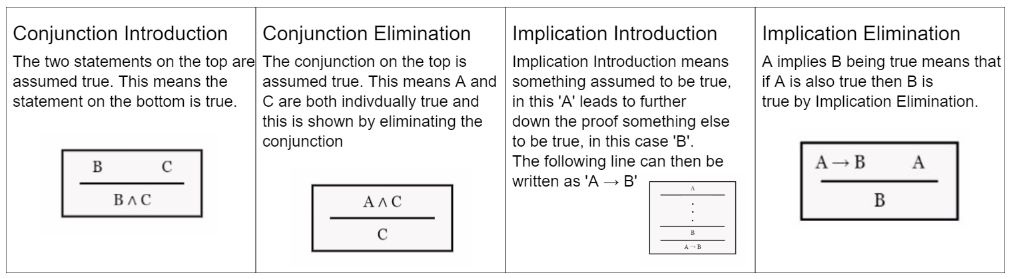
\includegraphics[scale=0.5]{hints}}
\caption{Format of hints given to the user on Level 6 when the questionnaire was completed}
\label{hints}
\end{figure}

For a game, it is important to have sufficient and helpful hints for the user so that the user feels that they are really benefiting by looking at hints and that it gives them enough help when looking at them. In hindsight, the hints need to be genuinely different and helpful, rather than just the repetition of the rules that were already displayed at the start of the level. From an educational perspective, hints can be crucial in the learning process. \cite{chen2009effects} Good hints could make the difference between a user carrying on with playing or giving up, so prompting the user with useful hints that they can then make progress with, may help them get over a barrier which otherwise they wouldn't be able to overcome and therefore give up and stop the game.   

A response from a user gave a nice suggestion on how to improve the hints system ``a better hint system that gives you a hint in to how the structure should be". The idea of displaying an empty proof structure with dots displayed is one that will be taken forward into further iterations of the code. As well as this, the algorithm that works out whether the proof entered by the user is correct could help to provide more support to let the user know which part of the proof is wrong. Helping users so they can overcome the problems they are facing during the game is one of the key qualities that a good game needs. All of this written feedback is helpful and a reworking of how the hints section works will be a suitable improvement to the system and help users overcome the difficulty they faced during the game.

Another suggestion was that the answer can be revealed if the user was stuck on a particular level. This would hopefully mean a user would be able to understand how the proof has been formed from seeing the answer and then the user can proceed onto the next level. By giving the user the answer, they would get no reward in the form of points for completing the level, but it will give them added knowledge of knowing how the level should be proved correctly.

\subsection{Levels and Difficulty}

Six levels were created for the users to work through on the game and it was interesting to see what stage people got to, how they thought that the difficulty increased as the levels progressed and if they didn't finish it, what the issue was. It was important that people could progress through the levels rather than giving up. If the user gave up, then they weren't learning so the game was not serving its purpose correctly. By getting users to 'do' things to learn, in this case formulating levels, kinaesthetic learning principles were being implemented, fulfilling a goal in Section \ref{goals}. Each level started by introducing a concept to the user, which they would then have to create a similar example, using the rules that had been displayed and taught.

5 people out of the 15 only managed to get to Level 2 of the game. This figure is a third of the people who played the game and one of the reasons that people didn't finish the game reveal that they didn't feel that they knew enough about the topic of Natural Deduction. This is the responsibility of the game to help guide the user and through a mixture of lack of support to the user and difficult concepts, it made the game unachievable for some. 

Responses for why users didn't complete the game included ``Could not work out how to complete the level correctly" and ``Couldn't answer Question 2, as I have no idea what proof it is wanting or how to prove it." Both of these statements allude to the same thing that the Natural Deduction theory wasn't explained clear enough and this greatly affected the progress of more novice users. This reaffirms the fact that a more comprehensive package of support is needed for users to make sure that everyone is capable of learning the material and successfully completing the levels.

More encouragingly 6 out of 15 users managed to get to Level 5 or further and 3 people completed the game. This shows that if users have the knowledge then it wasn't the gameplay and usability that was stopping them from progressing. The main thing that was stopping users that struggled with the game was a lack of understanding.

Difficulty of levels was a mixed issue from the participants of the survey. When creating a game it is important to get the level of difficulty correct between levels \cite{aponte2009scaling}. Some users commented with ``Levels increased nicely" and ``Good curve" whilst another user made the comment that ``The difficulty increased quickly for a novice" and also that ``Thought level 2 got too difficult too quickly". If users have had previous experience with Natural Deduction then it will probably be the case that they didn't think the difficulty curve was a difficult as to some beginners to Natural Deduction. This fact further highlights the lack of support for users that have not had experience of Natural Deduction logic and the need for more support to be given. 

\subsection{Fun}

Gamification and Fun go hand in hand with the aim of the principle of Gamification for the game players to learn something through playing a game which as a consequence is more fun than learning in other environments. Requirement \ref{ssection:fun9} highlighted the fact that this game should be more fun than learning in a traditional way.

If survey participants did not enjoy playing the game, or not realise it for what it is, which is to deliver education in a more exciting way, then the software has not delivered on key requirements. Enjoyment should be had, even though it is learning maths.

Gaming concepts such as a score system, multiple levels and interactive drag and drop have all been implemented and should all contribute to a fun experience for the user. The user was asked outright 'How fun did you find the game?'. The mean score for the game was 2.79/5 with a median score of 3. This is unexpectedly low but comments associated with the enjoyment of the game explained key reasons why it didn't fully entertain them.

One telling comment was that ``There's only so much fun you can find maths". This reignites the consideration that the game should have been created without the proper Natural Deduction notation. During this project, the importance has been highlighted that the software should be a valuable educational tool. Without proper notation or structure, the difficulty would be transferring the skills learnt in the game to more academic environments such as a classroom. By having the correct notation in place, it allows users to easily take what they have learnt away from the game and use it in other Mathematical or Computer Science disciplines such as the previously mentioned Lambda Calculus.

Another observation from a user was that ``It was quite good but it's still doing proofs which are boring". I think it's important to realise that this is a game that is suppose to teach Natural Deduction so although this particular user may find this boring, they may still find it more engaging and entertaining than learning Natural Deduction out of a book. For the first version of the game that was released, fun was not the most important priority and this can be improved with fine tuning of the user interface. 


\subsection{Educational Value} \label{ssection:edu}

One of the most important results of this project is whether the users thought they were learning and whether they thought there was value to playing the game and educating themselves in this way. Educational value of games was part of the reason this project was undertaken. If people thought that learning mathematical logic through gaming was valuable then this project will be worthwhile. 

Of the 15 people that answered the survey, it was asked about how effective the game was as an educational tool. It was encouraging to discover that the mean average score was 3.93/5. Over 70\% of participants ranked this a 4 or 5 for educational effectiveness which shows how people value this game as an educational resource. It shows that the majority of people thought the software was a positive educational experience. Along with the result that 86.7\% of participants in the survey thought they learnt more about Natural Deduction than they did previously, the users seemed to value the educational learning benefits that the game offers. Users suggests by the results that this game has great educational potential.

Yet more evidence points to the users feeling that they benefited educationally. 11 out of 15 users responded believed that this game is a better way to learn than learning by traditional methods like pen and paper or learning in a classroom. Also seven out of nine participants answered that they had no prior experience of Natural Deduction and that this game was a better way to learn that via traditional learning methods. This achieves Requirement \ref{ssection:fun9} which was to achieve a minimum threshold of 75\% of users preferring to use this game than learning manually. By having a high percentage of users that prefer to learn by games, it suggests that this game could be a feasible and more enjoyable way of learning.

\subsection{Usability}

Questions were asked to assess whether the user had a good experience and enjoyed the game they played. A user stopping playing because of usability issues is serious and harms the true reflection of the game's mathematical content. Some comments were received to that effect. This questionnaire is to pick out what does and doesn't work in the game and improve those parts. 

All of the drag and drop worked correctly and no users commented on unreliable drag and drop which is an important usability feature that was worked on extensively to get correct. A smooth drag and drop interface was important for the usability of the game. Also, all the buttons were sensible colours, meaning that actions remained intuitive for the user, with red displaying the 'Delete All' button and green having the 'Check Proof' button.

When asking users whether they thought the game was fun, one user stated that ``I found it really engaging because I wanted to keep going and reach more levels and complete the proofs and learn more rules, but the usability issues were really frustrating and it took me a long time to construct the proof for level 5 which I then did wrong because I misplaced one part of it. Starting again would have been frustrating so I stopped then". To have a user stop because of usability is just as bad as a user stopping because they are stuck. For whatever reason the user stops, this is the point that they are not learning, so the experience needs to be as pleasant as possible to make sure that the user doesn't give up.

A number of users complained about other usability issues. A popular topic was the lack of an undo button. ``An 'undo' button to take back the last step" was a common criticism from users. This meant that if users made a mistake on the proof then instead of being to undo that move, they had to start again and create a new proof structure. Whilst an undo button may be hard to implement, other solutions may be explored to solve this issue.

The game being time consuming was a reason that users didn't complete the game. A slightly more usable and slick program may have improved perceptions of the game and users would have not given up as easily. One strong usability point is that the game only used a mouse. Removing the keyboard made it easier for the user to navigate the game as they wouldn't get confused by a mixture of keyboard and mouse input.

%As usability is one of the largest outstanding issues with the game which has not been discussed at great length in this project, some reading was done to pinpoint exactly where this specific %project could be improved. 

\section{Improvements to the game}

Following feedback received from the game, there were a number of small bugs which were fixed. This included temperamental display of the hints and the 'Not Correct' boxes displaying unhelpful tips on how the level can be solved. Both these bugs have been fixed and will improve the support that is given to the user.

Other minor bugs that were fixed had usability in mind. A slight movement when the users picked up an object where 2 or more objects were on the same point has been fixed. The software needed to pinpoint which object was being picked up to stop this issue. Another small feature that has been improved which will enhance user experience is that the outline of the proof structure or statement will go turn red when they drag the shape to the bin and it is hovering over it.  

Since the conclusion of the survey, a number of issues have more substantially changed to improve user experience. Firstly the hints have become more useful. Now one of the boxes displaying hints contains an empty proof structure, giving the user a structure which they can recreate on screen and then input the correct statements. This was important to add to the game because one of the key sticking points was that the user did not know what to do. By giving the user more prompts, it makes it more accessible and helps the user complete the game. Another one of the hints boxes gives the user more information about the level, helping them further.

The rules are now permanently displayed. This was done with education in mind. One of the strengths of the game needs to be that they are learning all the time. By presenting the rules to the user that are available at all times, the rules are always in front of them. This should reinforce the knowledge that the user is learning because of the ever presence of the rules. This are the educational parts that the user has received at the start of each level, so it is not new material for the user. Displaying this at all times will hopefully improve knowledge that is retained because of the repetition of the user seeing the rule.

\section{Further Work}

Taking into account the users' comments as well as my own thoughts on the project, here are are some features that I'd like to implement in the future.
 
Users expressed an interest in an undo button so that they could alter proofs once they have connected them. Users commented that when making mistakes, the process was tedious to create a whole new proof structure when an undo button could be implemented. Implementing an undo button would be hard as it would take a lot of space to store all of the individual moves the user made. It shouldn't be too difficult to implement an undo button for one move though, where a snapshot of the previous move is stored which the user can revert to. It should also be made possible that users can drag statements over existing statements to replace them. This will reduces the need for an undo button in a number of cases and give the user an alternative option. There would still be the need for an undo button when two proof structures are dragged together as this cannot be undone. An undo button would be suitable for this purpose and should be implemented for this reason.

An additional improvement that could be made to the usability of the game is when users have acquired a particular bit of knowledge and are practised at it, parts of proofs are automatically entered for the user. Once a user has mastered a still, they shouldn't have to go through the process of creating this every time and therefore variables should filter through the structure of the proof. This would reduce the time it takes for the user to complete levels. This would be useful, especially for longer levels. Manual structuring of basic moves when solving complicated levels would get repetitive and dull. By making sure that the user doesn't have to perform every step, it will keep enjoyment high as simpler moves will be automated.

Some users commented that dragging the buttons straight away would be a more natural approach rather than clicking the button and then having to move the cursor to pick up the item. A future feature could be that the buttons are on the canvas and that this does indeed happen. When they click down on the button, users will be able to drag straight from that location to give them a more intuitive feel.

By having the Natural Deduction proof system in place, it allows further opportunity for a larger variety of logic systems Firstly, more complicated levels could be created with the intuitionistic logic. Once a solid set of levels has been created for this, the software has the potential to introduce other logical systems like Classical logic. A step to realising this feature is allowing users to create their own levels. If the user can create and save their own levels, it makes the software more open and allows greater use of the software by more experience logicians. Only a finite number of logical symbols would need to be permitted for a large range of levels to be created in a large amount of logics systems. Symbols like the existential quantification (there exists) and turnstile (provable) would needed to be added so that the user can create more complicated levels.